\documentclass[11pt,a4paper]{article}

\usepackage[utf8]{inputenc}
\usepackage[T1]{fontenc}
\usepackage{geometry}
\geometry{
  a4paper,
  top=0.95in,
  bottom=0.95in,
  left=0.95in,
  right=0.95in
}

\usepackage{lmodern}
\usepackage{amsmath,amssymb}
\usepackage{graphicx}
\usepackage{booktabs}
\usepackage{array}
\usepackage{tabularx}
\usepackage{enumitem}
\usepackage{fancyhdr}
\usepackage{xcolor}
\usepackage{listings}
\usepackage{microtype}
\usepackage{tikz}
\usetikzlibrary{shapes.geometric,arrows.meta,positioning,fit,backgrounds,calc,chains,shadows}
\usepackage[most]{tcolorbox}
\usepackage[colorlinks=true,linkcolor=navyBlue,citecolor=navyBlue,urlcolor=navyBlue]{hyperref}

% --- Color Palette (Matching Systems Lab / Shobdomala Design Philosophy) ---
\definecolor{navyBlue}{RGB}{11, 59, 96}
\definecolor{headerBlue}{RGB}{15, 76, 129}
\definecolor{accentCyan}{RGB}{6, 182, 212}
\definecolor{lightGrayBg}{RGB}{248, 250, 252}
\definecolor{borderGray}{RGB}{226, 232, 240}
\definecolor{boxHeader}{RGB}{23, 70, 115}
\definecolor{codeKw}{RGB}{147, 51, 234}
\definecolor{codeComment}{RGB}{100, 116, 139}
\definecolor{codeString}{RGB}{13, 148, 136}

% --- Custom Header & Footer ---
\pagestyle{fancy}
\fancyhf{}
\fancyhead[L]{\small\scshape KeyPressMonitor}
\fancyhead[R]{\small\scshape Systems Lab — Assignment 4}
\fancyfoot[C]{\thepage}
\renewcommand{\headrulewidth}{0.5pt}
\renewcommand{\footrulewidth}{0.0pt}

% --- Section Styling ---
\usepackage{titlesec}
\titleformat{\section}{\color{navyBlue}\normalfont\Large\bfseries}{\thesection}{1em}{}
\titleformat{\subsection}{\color{navyBlue}\normalfont\large\bfseries}{\thesubsection}{1em}{}
\titleformat{\subsubsection}{\color{navyBlue}\normalfont\normalsize\bfseries}{\thesubsubsection}{1em}{}

% --- TColorBox Styling ---
\tcbset{
  labbox/.style={
    enhanced,
    colback=lightGrayBg,
    colframe=navyBlue,
    fonttitle=\bfseries\color{white},
    coltitle=white,
    colbacktitle=navyBlue,
    boxrule=0.8pt,
    arc=3pt,
    left=10pt,
    right=10pt,
    top=8pt,
    bottom=8pt,
    titlerule=0.5pt
  }
}

% --- Code Listings Styling ---
\lstdefinestyle{masmstyle}{
  backgroundcolor=\color{lightGrayBg},
  commentstyle=\color{codeComment}\itshape,
  keywordstyle=\color{navyBlue}\bfseries,
  stringstyle=\color{codeString},
  basicstyle=\ttfamily\footnotesize,
  breakatwhitespace=false,
  breaklines=true,
  captionpos=b,
  keepspaces=true,
  numbers=left,
  numbersep=8pt,
  numberstyle=\tiny\color{codeComment},
  showspaces=false,
  showstringspaces=false,
  showtabs=false,
  tabsize=2,
  frame=single,
  rulecolor=\color{borderGray}
}
\lstset{style=masmstyle}

\begin{document}

% ==============================================================================
% TITLE & METADATA BLOCK
% ==============================================================================

\begin{center}
  {\Huge\textbf{\color{navyBlue}KeyPressMonitor}}\\[0.25em]
  {\Large\textbf{Real-Time Keystroke Telemetry, Ergonomic Analytics, and Multi-Tier Input Suite in 32-bit MASM Assembly}}\\[0.8em]
  {\large Systems Lab Group Project — Assignment 4}\\[0.3em]
  {\small\textit{“Develop a real-time keyboard press monitor to display last N words typed, vowel/consonant proportions, and per-character frequencies”}}
\end{center}

\vspace{0.8em}
\noindent\rule{\textwidth}{1.2pt}
\vspace{0.8em}

\noindent
\begin{minipage}[t]{0.48\textwidth}
  \begin{tcolorbox}[labbox, title=Dept. of Computer Science \& Engineering, colbacktitle=navyBlue]
    \textbf{Jadavpur University}\\[0.5em]
    \begin{tabular}{ll}
      \textbf{Course}     & Systems Lab \\
      \textbf{Year}       & 2025–2026 \\
      \textbf{Semester}   & 5th (Odd) \\
      \textbf{Group No.}  & 1 \\
      \textbf{Supervisor} & Prof. Anasua Sarkar
    \end{tabular}
  \end{tcolorbox}
\end{minipage}
\hfill
\begin{minipage}[t]{0.48\textwidth}
  \begin{tcolorbox}[labbox, title=Group Members \& Roll Numbers, colbacktitle=navyBlue]
    \centering
    \begin{tabular}{ll}
      \toprule
      \textbf{Group Member} & \textbf{Roll No.} \\
      \midrule
      Aritra Dutta       & 002410501009 \\
      Subham Bhat        & 002410501020 \\
      Antariksh Sengupta & 002410501028 \\
      Hrishikesh Bhanja  & 002410501030 \\
      Soham Neogi        & 002410501031 \\
      \bottomrule
    \end{tabular}
  \end{tcolorbox}
\end{minipage}

\vspace{0.6em}
\noindent
\begin{center}
\small
\begin{tabularx}{\textwidth}{lX}
  \toprule
  \textbf{Repository} & \url{https://github.com/Aricode2005/KeyPressMonitor} \\
  \textbf{Languages}  & 32-bit x86 MASM Assembly (\texttt{.386}, \texttt{.387}), JavaScript (Manifest V3), C++17 (\texttt{WH\_KEYBOARD\_LL}) \\
  \textbf{Platform}   & Windows 10/11 (\texttt{kernel32.lib} only); Chrome Extension (Windows/macOS/Linux) \\
  \textbf{Source Size}& $\approx 12,000$ lines of code across 22 modular source files \\
  \textbf{Self-Test}  & 19 automated internal assertion test cases (\texttt{KeyMonitor.exe /selftest}), 100\% passing \\
  \bottomrule
\end{tabularx}
\end{center}

\vspace{0.5em}
\tableofcontents
\newpage

% ==============================================================================
% SECTION 1: INTRODUCTION & PROBLEM STATEMENT
% ==============================================================================
\section{Introduction}

\subsection{Problem Statement and Core Objectives}
The fundamental objective of Assignment 4 is the construction of a real-time keyboard monitoring system implemented in assembly language. In traditional systems programming pedagogy, such utilities often devolve into trivial command-line loops reading single characters from standard input. However, in modern operating system environments, real-time keyboard telemetry poses significant systems-level challenges:
\begin{enumerate}[leftmargin=*]
  \item \textbf{Low-Level Input Interception}: Asynchronously capturing keyboard transitions without blocking the main rendering loop or locking system resources.
  \item \textbf{High-Fidelity Frequency Tracking}: Maintaining frequency counters for all 256 ASCII states, word delimitation, and ratio calculations (vowels vs. consonants).
  \item \textbf{Circular Buffer Maintenance}: Managing a variable-length rolling buffer of the last $N$ keystrokes ($8 \le N \le 64$) with $O(1)$ amortized updates.
  \item \textbf{Zero-Flicker Visual Presentation}: Refreshing a complex multi-panel dashboard containing sparklines, gradients, and histograms without the visible flicker inherent in standard console clear-and-draw routines.
\end{enumerate}

% ==============================================================================
% SECTION 2: SYSTEM ARCHITECTURE & WHERE THE MONITOR SITS
% ==============================================================================
\section{System Architecture and Input Pipelines}

KeyPressMonitor is structured across a three-tiered execution model that bridges bare-metal Win32 console execution with global operating system hooks and browser-level telemetry.

\subsection{End-to-End Architectural Model Diagram}

\begin{figure}[htbp]
\centering
\noindent\resizebox{\textwidth}{!}{%
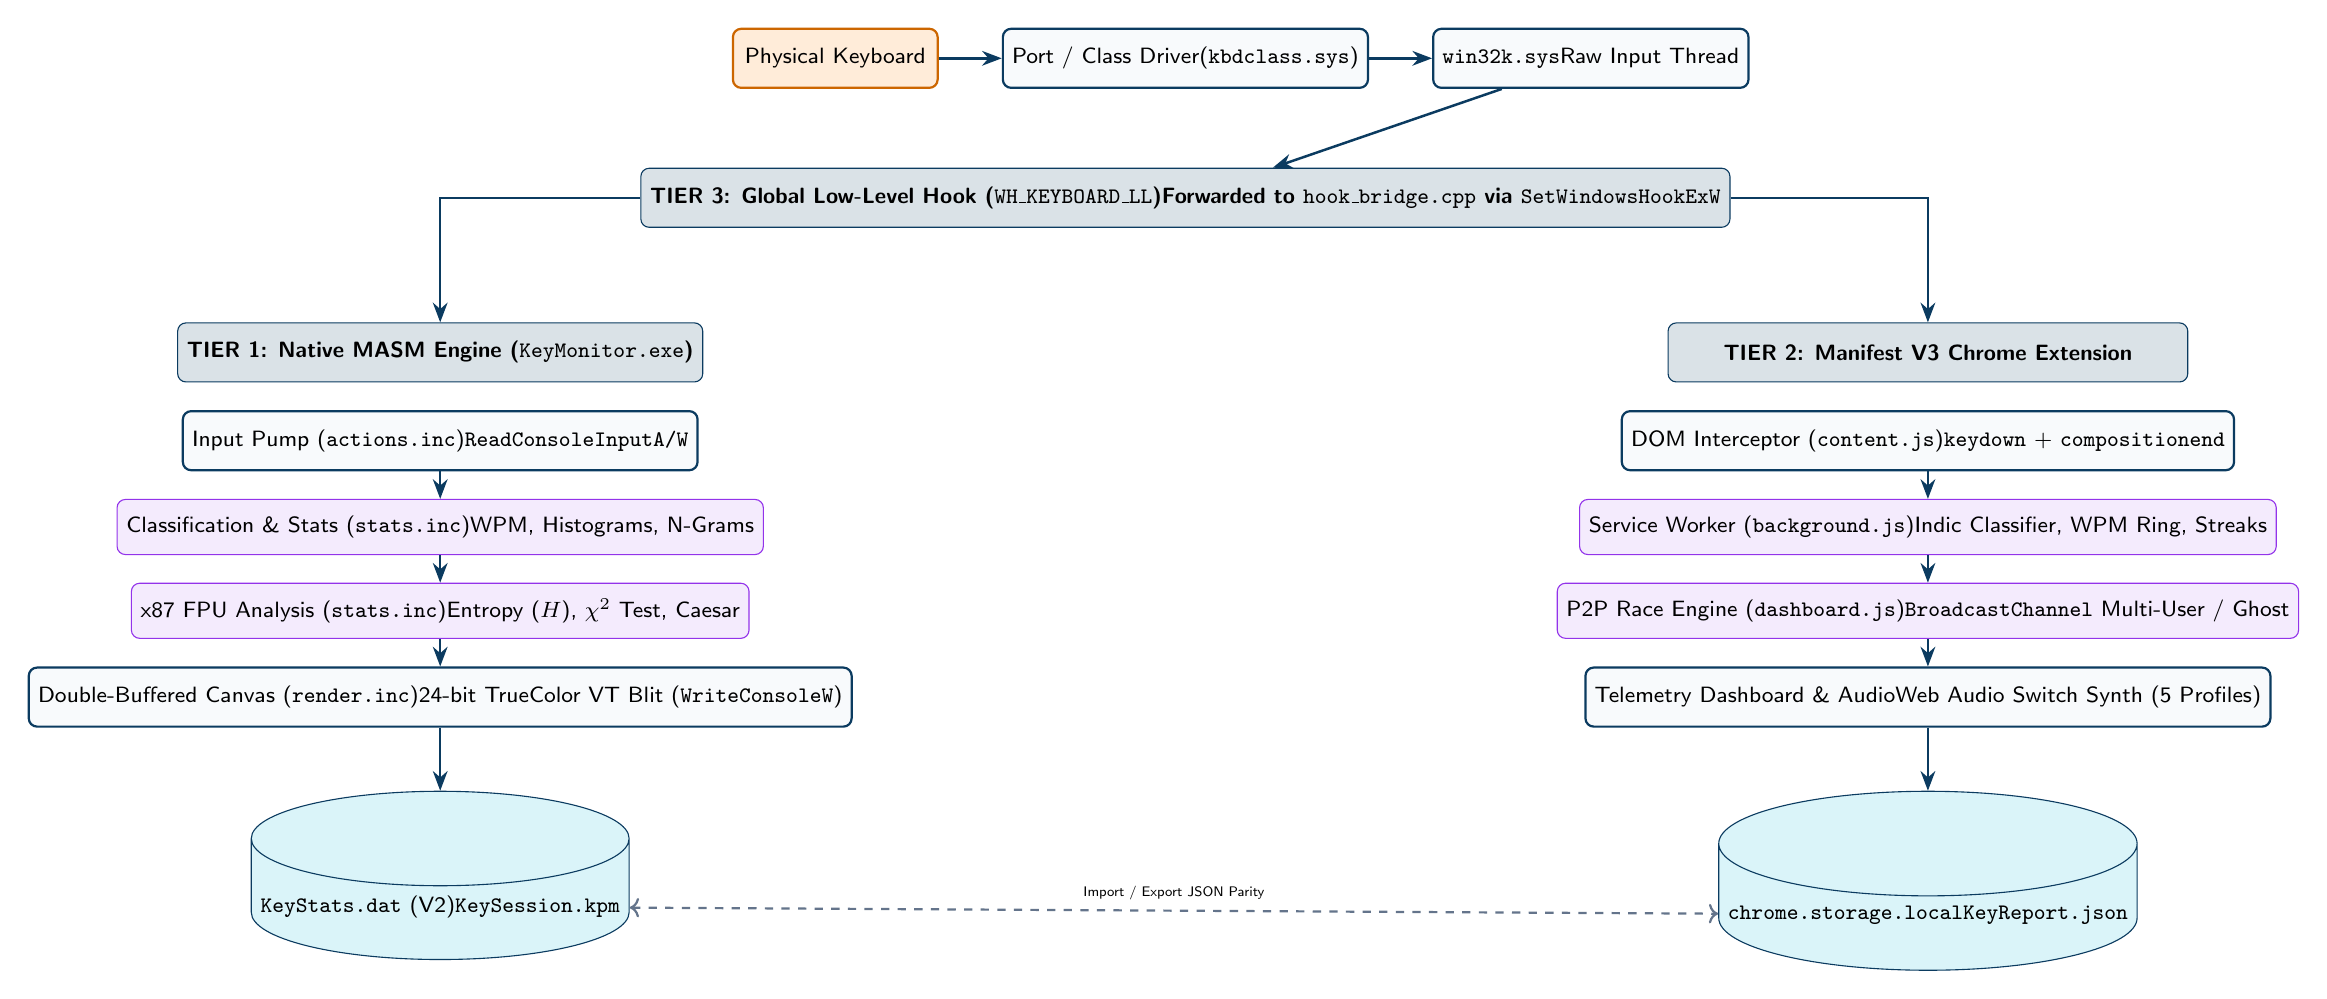
\begin{tikzpicture}[
  node distance=1.0cm and 0.8cm,
  font=\sffamily\footnotesize,
  box/.style={rectangle, draw=navyBlue, fill=lightGrayBg, rounded corners=3pt, text centered, minimum height=0.75cm, minimum width=2.6cm, line width=0.8pt},
  hdrbox/.style={rectangle, draw=navyBlue, fill=navyBlue!15, rounded corners=3pt, text centered, font=\sffamily\bfseries\footnotesize, minimum height=0.75cm, minimum width=2.8cm},
  action/.style={rectangle, draw=codeKw, fill=codeKw!10, rounded corners=3pt, text centered, minimum height=0.7cm, minimum width=2.5cm},
  storage/.style={cylinder, draw=navyBlue, fill=accentCyan!15, shape border rotate=90, aspect=0.25, text centered, minimum height=0.85cm, minimum width=2.6cm},
  arrow/.style={-{Stealth[length=2.5mm]}, line width=0.9pt, draw=navyBlue},
  darrow/.style={-{Stealth[length=2.5mm]}, dashed, line width=0.8pt, draw=codeComment}
]

  % Row 1: Hardware & Driver
  \node[box, fill=orange!15, draw=orange!80!black] (hw) {Physical Keyboard};
  \node[box, right=0.8cm of hw] (driver) {Port / Class Driver\\(\texttt{kbdclass.sys})};
  \node[box, right=0.8cm of driver] (raw) {\texttt{win32k.sys}\\Raw Input Thread};

  % Row 2: Hook & Dispatch
  \node[hdrbox, below=1.0cm of driver, minimum width=7.2cm] (hook) {TIER 3: Global Low-Level Hook (\texttt{WH\_KEYBOARD\_LL})\\Forwarded to \texttt{hook\_bridge.cpp} via \texttt{SetWindowsHookExW}};

  % Row 3: Two main tiers
  \node[hdrbox, below left=1.2cm and -0.8cm of hook, minimum width=6.6cm] (t1hdr) {TIER 1: Native MASM Engine (\texttt{KeyMonitor.exe})};
  \node[hdrbox, below right=1.2cm and -0.8cm of hook, minimum width=6.6cm] (t2hdr) {TIER 2: Manifest V3 Chrome Extension};

  % Tier 1 internals
  \node[box, below=0.35cm of t1hdr] (t1in) {Input Pump (\texttt{actions.inc})\\\texttt{ReadConsoleInputA/W}};
  \node[action, below=0.35cm of t1in] (t1calc) {Classification \& Stats (\texttt{stats.inc})\\WPM, Histograms, N-Grams};
  \node[action, below=0.35cm of t1calc] (t1fpu) {x87 FPU Analysis (\texttt{stats.inc})\\Entropy ($H$), $\chi^2$ Test, Caesar};
  \node[box, below=0.35cm of t1fpu] (t1rend) {Double-Buffered Canvas (\texttt{render.inc})\\24-bit TrueColor VT Blit (\texttt{WriteConsoleW})};

  % Tier 2 internals
  \node[box, below=0.35cm of t2hdr] (t2in) {DOM Interceptor (\texttt{content.js})\\\texttt{keydown} + \texttt{compositionend}};
  \node[action, below=0.35cm of t2in] (t2bg) {Service Worker (\texttt{background.js})\\Indic Classifier, WPM Ring, Streaks};
  \node[action, below=0.35cm of t2bg] (t2race) {P2P Race Engine (\texttt{dashboard.js})\\\texttt{BroadcastChannel} Multi-User / Ghost};
  \node[box, below=0.35cm of t2race] (t2ui) {Telemetry Dashboard \& Audio\\Web Audio Switch Synth (5 Profiles)};

  % Storage Tier
  \node[storage, below=0.8cm of t1rend] (store1) {\texttt{KeyStats.dat} (V2)\\\texttt{KeySession.kpm}};
  \node[storage, below=0.8cm of t2ui] (store2) {\texttt{chrome.storage.local}\\\texttt{KeyReport.json}};

  % Connections
  \draw[arrow] (hw) -- (driver);
  \draw[arrow] (driver) -- (raw);
  \draw[arrow] (raw) -- (hook);
  \draw[arrow] (hook) -| (t1hdr);
  \draw[arrow] (hook) -| (t2hdr);

  \draw[arrow] (t1in) -- (t1calc);
  \draw[arrow] (t1calc) -- (t1fpu);
  \draw[arrow] (t1fpu) -- (t1rend);
  \draw[arrow] (t1rend) -- (store1);

  \draw[arrow] (t2in) -- (t2bg);
  \draw[arrow] (t2bg) -- (t2race);
  \draw[arrow] (t2race) -- (t2ui);
  \draw[arrow] (t2ui) -- (store2);

  % Inter-tier JSON bridge
  \draw[darrow, <->] (store1) -- node[above, font=\sffamily\tiny] {Import / Export JSON Parity} (store2);

\end{tikzpicture}%
}
\caption{System architecture diagram depicting input interception, dual telemetry engines, and data storage.}
\label{fig:arch_model}
\end{figure}

\subsection{Modular Subsystem Breakdown}
The native assembly codebase is organized into ten discrete, decoupled include modules within \texttt{src/}:
\begin{itemize}[leftmargin=*]
  \item \textbf{\texttt{defs.inc}}: Win32 API prototypes, virtual key definitions (\texttt{VK\_*}), color constants, and binary magic signatures (\texttt{STAT\_MAGIC\_V1}, \texttt{STAT\_MAGIC\_V2}).
  \item \textbf{\texttt{data.inc}}: Global state variables, frequency arrays, theme color ramps, and precomputed trigonometric/logarithmic constants.
  \item \textbf{\texttt{render.inc}}: Canvas memory model ($100 \times 30$ character cells), RGB linear color interpolation (\texttt{Lerp}), and atomic ANSI VT escape sequence generation.
  \item \textbf{\texttt{stats.inc}}: Character classification (vowels, consonants, digits, whitespace, symbols), n-gram frequency counters, and live WPM sliding window math.
  \item \textbf{\texttt{session.inc}}: Binary persistence subsystem handling backwards-compatible \texttt{KeyStats.dat} loading, session recording (\texttt{KeySession.kpm}), and ghost race timing (\texttt{KeyGhost.dat}).
  \item \textbf{\texttt{dashboard.inc}}: UI rendering routines for the primary telemetry dashboard, typing test interface, biomechanics screen, and help overlay.
  \item \textbf{\texttt{reports.inc}}: Text, CSV, and HTML document generators featuring standalone SVG sparklines.
  \item \textbf{\texttt{actions.inc}}: Event routing, keyboard/mouse input decoding, and JSON report export engine.
  \item \textbf{\texttt{console.inc}}: Low-level console screen buffer configuration, cursor visibility control, and graceful cleanup handlers.
  \item \textbf{\texttt{selftest.inc}}: Automated 19-point assertion test suite executing without GUI intervention.
\end{itemize}

% ==============================================================================
% SECTION 3: COWORKER SUBSYSTEM CONTRIBUTIONS IN DETAIL
% ==============================================================================
\section{In-Depth Coworker Subsystem Implementations}

The KeyPressMonitor architecture was partitioned into dedicated functional domains. The core subsystems engineered by group members are detailed below:

\subsection{Subham Bhat: Mathematical Modeling, Information Theory \& Cryptanalysis}
Subham Bhat authored the analytical, statistical, and cryptanalytic components housed in \texttt{src/stats.inc}:

\subsubsection{Hardware x87 Shannon Entropy Engine (\texttt{FYL2X})}
Evaluating information entropy over the alphabet requires calculating:
\begin{equation}
  H(X) = -\sum_{i=1}^{26} p(x_i) \log_2 p(x_i) \quad \text{with } p(x_i) = \frac{c_i}{n}
\end{equation}
Floating-point division of small probabilities introduces compounding truncation errors. Subham algebraically refactored this into:
\begin{equation}
  H(X) = \log_2(n) - \frac{1}{n}\sum_{i=1}^{26} c_i \log_2(c_i)
\end{equation}
Using the x87 FPU coprocessor instruction \texttt{FYL2X} ($y \cdot \log_2 x$), the calculation evaluates directly on hardware:
\begin{lstlisting}[language={[x86masm]Assembler}]
fldz                                ; ST(0) = 0.0 (accumulator)
xor  esi, esi
at_h:
cmp  taCnt[esi*4], 0
je   at_hnext
fild taCnt[esi*4]                   ; Push c_i
fild taCnt[esi*4]                   ; Push c_i
fyl2x                               ; ST(0) = c_i * log2(c_i)
faddp st(1), st                     ; Accumulate
at_hnext:
inc  esi
cmp  esi, 26
jb   at_h
fild taN                            ; Push n
fdivp st(1), st                     ; sum / n
fld1
fild taN
fyl2x                               ; 1.0 * log2(n)
fsubrp st(1), st                    ; log2(n) - (sum / n)
fmul fHundred                      ; Multiply by 100 for fixed-point integer display
fistp taH100                        ; Store integer scaled entropy
\end{lstlisting}

\subsubsection{Pearson $\chi^2$ Goodness-of-Fit and Caesar Cryptanalysis}
Subham implemented Pearson's $\chi^2$ test against standard English monograph shares ($E_i$):
\begin{equation}
  \chi^2 = \sum_{i=1}^{26} \frac{(O_i - E_i)^2}{E_i}
\end{equation}
With 25 degrees of freedom at $\alpha = 0.05$, the critical value is $\chi^2_{\text{crit}} = 37.65$. For automated cryptanalysis, the engine sweeps all 26 modular shifts $k \in [0, 25]$:
\begin{equation}
  C_k = \sum_{i=1}^{26} \frac{(O_{(i+k)\bmod 26} - E_i)^2}{E_i}
\end{equation}
The shift $k$ that minimizes $C_k$ is identified as the Caesar cipher rotation, automatically deciphering ROT-$n$ encoded text.

\subsubsection{N-Gram Matrices}
Subham implemented two rolling hash transition matrices:
\begin{itemize}[leftmargin=*]
  \item \textbf{Bigrams}: $26 \times 26 = 676$ \texttt{DWORD} counters indexed via $\text{Index} = (\text{prev} \times 26) + \text{curr}$.
  \item \textbf{Trigrams}: $26^3 = 17,576$ \texttt{DWORD} counters ($70,304\text{ bytes}$) indexed via $\text{Index} = ((\text{prev}_2 \times 26) + \text{prev}_1) \times 26 + \text{curr}$.
\end{itemize}

\subsection{Aritra Dutta: Graphics Pipeline, VT-100 Canvas \& Thermal Color Blending}
Aritra Dutta engineered the zero-flicker graphics pipeline and console interface in \texttt{src/render.inc} and \texttt{src/console.inc}:

\subsubsection{Double-Buffered Memory Canvas ($100 \times 30 \times 12\text{ bytes}$)}
To eliminate visual tearing, Aritra built an offscreen memory canvas:
\begin{equation}
  \text{Canvas Size} = 100 \times 30 \times 12\text{ bytes} = 36,000\text{ bytes}
\end{equation}
Each cell packs character glyph, 24-bit TrueColor foreground (\texttt{0x00RRGGBB}), and 24-bit background. Cell clipping protects boundaries, and \texttt{C\_KEEP} preserves existing background colors during alpha-like blits.

\subsubsection{Atomic Virtual Terminal Stream Flush}
In \texttt{FlushCanvas}, Aritra implemented an engine that formats the frame buffer into UTF-16 ANSI VT sequences:
\begin{equation}
  \texttt{\textbackslash x1b[38;2;R;G;Bm}\quad \text{(Foreground)}\quad\text{and}\quad\texttt{\textbackslash x1b[48;2;R;G;Bm}\quad \text{(Background)}
\end{equation}
The entire frame buffer is emitted to standard output in a single call to \texttt{WriteConsoleW}, delivering a smooth, flicker-free $60\text{ FPS}$ interface. For legacy terminals, Aritra added an Euclidean palette fallback mapping TrueColor values to the nearest matching 16-color attribute.

\subsubsection{Linear Color Blending (\texttt{Lerp}) and Multi-Stop Heat Ramps}
Aritra designed fixed-point integer linear interpolation:
\begin{equation}
  R_{\text{new}} = R_1 + \frac{(R_2 - R_1) \times f_{256}}{256}
\end{equation}
This powers dynamic thermal gradients for the heatmap, transitioning keys through Cold Blue $\rightarrow$ Cyan $\rightarrow$ Green $\rightarrow$ Yellow $\rightarrow$ Amber $\rightarrow$ Hot Red.

\subsection{Hrishikesh Bhanja: Typing Test Engine, Ghost Timing \& Session Serialization}
Hrishikesh Bhanja designed the interactive typing test engine, ghost racing, and session recording in \texttt{src/session.inc}:

\subsubsection{Multi-Category Typing Test Engine}
Hrishikesh constructed the typing test harness featuring four test categories (\texttt{STANDARD}, \texttt{QUOTES}, \texttt{CODE}, and \texttt{NUMBERS}) across 12 distinct preset challenges. The test tracks character-by-character accuracy, keystroke errors, and real-time WPM.

\subsubsection{Live Ghost Racing (\texttt{KeyGhost.dat})}
To challenge the typist, Hrishikesh implemented high-resolution ghost tracking:
\begin{itemize}[leftmargin=*]
  \item \textbf{Trajectory Recording (\texttt{GhostMark})}: At each character index $i$, \texttt{GetTickCount} records millisecond offsets: $\texttt{testTimes}[i] = t_{\text{curr}} - t_{\text{start}}$.
  \item \textbf{Persistence (\texttt{KeyGhost.dat})}: When a sentence completes, \texttt{GhostFinish} compares the run against the personal best, serializing faster trajectories under signature \texttt{"KPMG"}.
  \item \textbf{Pacing Indicator (\texttt{GhostPos})}: During live runs, a ghost cursor ($\blacktriangle$) tracks progress in real time, showing whether the typist is ahead or behind their record.
\end{itemize}

\subsubsection{Packed 32-bit Keystroke Session Recording and Replay Engine}
Hrishikesh created \texttt{SaveSession}, recording up to 32,768 keystrokes into \texttt{KeySession.kpm}. Each entry encodes character, virtual key code, and millisecond delta into a compact 32-bit field:
\begin{equation}
  \text{Entry} = (\text{char} \ \& \ \texttt{0xFF}) \ \vert \ ((\text{VK} \ \& \ \texttt{0xFF}) \ll 8) \ \vert \ ((\Delta t \ \& \ \texttt{0xFFFF}) \ll 16)
\end{equation}
Pressing \texttt{F10} activates \texttt{StartReplay}, deterministically replaying the typing session at exact real-world speed.

\subsection{Soham Neogi: Biomechanics Engine, Sound Synthesis \& Gamification}
Soham Neogi authored the ergonomic strain models, audio synthesis, and gamification logic in \texttt{src/stats.inc} and the Chrome Extension:

\subsubsection{Biomechanical Load and Fatigue Modeling}
Soham built the anatomical tracking matrix:
\begin{itemize}[leftmargin=*]
  \item \textbf{Hand Balance and Alternation}: Tracking left vs. right hand load and measuring alternation percentage ($N_{\text{alt}} / N_{\text{total}}$) to gauge rhythm consistency.
  \item \textbf{8-Finger Ergonomic Distribution}: Mapping keys to specific fingers (Left/Right Pinky, Ring, Middle, Index, and Thumbs).
  \item \textbf{Row Fatigue Index}: Profiling usage across Number, Top, Home, Bottom, and Space rows.
\end{itemize}

\subsubsection{Dual-Mode Sound Synthesis}
Soham implemented responsive audio feedback:
\begin{itemize}[leftmargin=*]
  \item \textbf{MASM Core}: Calling \texttt{kernel32!Beep} parameterized by virtual key code ($f = 750 + (\text{VK} \bmod 16) \times 35\text{ Hz}$).
  \item \textbf{Web Audio Engine}: Synthesizing five distinct mechanical switch profiles: Cherry MX Blue (tactile click leaf), MX Brown (cushioned thock), IBM Model M (buckling spring ping), Typewriter (mechanical striker + bell), and Sci-Fi Blaster (frequency-swept square wave).
\end{itemize}

\subsubsection{Dynamic Streak Multipliers and XP Gamification}
Soham designed the progression engine:
\begin{equation}
  \text{XP} = \text{TotalKeys} + (\text{BestStreak} \times 2) + (\text{PeakWPM} \times 3) + (\text{UnlockedBadges} \times 100)
\end{equation}
Awarding ranks (\texttt{NOVICE} to \texttt{GRANDMASTER}) and 8 achievement badges (e.g. Centurion, Velocity Demon, Polyglot Typist).

% ==============================================================================
% SECTION 4: DATA VERSIONING (KPM1 -> KPM2)
% ==============================================================================
\section{Binary Data Serialization and Schema Versioning}

Persisting data via direct binary dumps (\texttt{WriteFile}) saves exact struct layouts. When schema definitions evolve without version identifiers, loading legacy binary files causes buffer under-reads and structural misalignment.

To ensure strict backwards compatibility, \textbf{Antariksh Sengupta} introduced dual-magic signatures in \texttt{src/defs.inc}:
\begin{lstlisting}[language={[x86masm]Assembler}]
STAT_N_V1     EQU 12          ; Legacy v1 DWORD count (48 bytes)
STAT_MAGIC_V1 EQU 314D504Bh   ; "KPM1" in little-endian ASCII
STAT_N        EQU 16          ; Modern v2 DWORD count (64 bytes)
STAT_MAGIC    EQU 324D504Bh   ; "KPM2" in little-endian ASCII
\end{lstlisting}

\begin{table}[htbp]
\centering
\small
\begin{tabularx}{\textwidth}{lllX}
  \toprule
  \textbf{Offset} & \textbf{Field Constant} & \textbf{Type} & \textbf{Description} \\
  \midrule
  \texttt{0x00} & \texttt{ST\_MAGIC}   & \texttt{DWORD} & Format identifier (\texttt{"KPM1"} or \texttt{"KPM2"}) \\
  \texttt{0x04} & \texttt{ST\_TOTAL}   & \texttt{DWORD} & Cumulative session keystrokes \\
  \texttt{0x08} & \texttt{ST\_VOW}     & \texttt{DWORD} & Total vowels count \\
  \texttt{0x0C} & \texttt{ST\_CON}     & \texttt{DWORD} & Total consonants count \\
  \texttt{0x10} & \texttt{ST\_WORDS}   & \texttt{DWORD} & Delimited words typed \\
  \texttt{0x14} & \texttt{ST\_PEAK}    & \texttt{DWORD} & Session peak WPM \\
  \texttt{0x18} & \texttt{ST\_AVG}     & \texttt{DWORD} & Session average WPM \\
  \texttt{0x1C} & \texttt{ST\_TIME}    & \texttt{DWORD} & Total active elapsed seconds \\
  \texttt{0x20} & \texttt{ST\_BS}      & \texttt{DWORD} & Backspace deletion count \\
  \texttt{0x24} & \texttt{ST\_BEST}    & \texttt{DWORD} & All-time personal best peak WPM \\
  \texttt{0x28} & \texttt{ST\_TBEST}   & \texttt{DWORD} & All-time typing test velocity record \\
  \texttt{0x2C} & \texttt{ST\_SESS}    & \texttt{DWORD} & Total completed sessions counter \\
  \midrule
  \texttt{0x30} & \texttt{ST\_VERSION} & \texttt{DWORD} & Explicit schema revision (Value = \texttt{2}) \\
  \texttt{0x34} & \texttt{ST\_IND\_VOW}& \texttt{DWORD} & Indic script independent vowels + matras \\
  \texttt{0x38} & \texttt{ST\_IND\_CON}& \texttt{DWORD} & Indic script consonants \\
  \texttt{0x3C} & \texttt{ST\_RESERVED}& \texttt{DWORD} & Reserved alignment padding for future extensions \\
  \bottomrule
\end{tabularx}
\caption{Binary record memory layout for \texttt{KeyStats.dat} comparing V1 (lines 1–12) and V2 (lines 1–16).}
\label{tab:keystats}
\end{table}

In \texttt{src/session.inc}, \texttt{LoadStats} validates the header:
\begin{lstlisting}[language={[x86masm]Assembler}]
LoadStats PROC USES ebx
    invoke CreateFileA, ADDR sStatsFile, 80000000h, 1, 0, 3, 80h, 0
    cmp  eax, -1
    je   ls_done
    mov  ebx, eax
    invoke ReadFile, ebx, ADDR lastStats, STAT_N * 4, ADDR nRead, 0
    invoke CloseHandle, ebx

    cmp  nRead, STAT_N * 4
    jne  ls_check_v1
    cmp  lastStats, STAT_MAGIC
    je   ls_valid

ls_check_v1:
    cmp  nRead, STAT_N_V1 * 4
    jne  ls_done
    cmp  lastStats, STAT_MAGIC_V1
    jne  ls_done
    ; In-memory zero-extension migration
    mov  lastStats[ST_VERSION*4], 1
    mov  lastStats[ST_IND_VOW*4], 0
    mov  lastStats[ST_IND_CON*4], 0
    mov  lastStats[ST_RESERVED*4], 0

ls_valid:
    mov  hasLast, 1
    mov  eax, lastStats[ST_BEST*4]
    mov  bestPeakAll, eax
    mov  eax, lastStats[ST_TBEST*4]
    mov  bestTestAll, eax
ls_done:
    ret
LoadStats ENDP
\end{lstlisting}

% ==============================================================================
% SECTION 5: INDIC SCRIPT SUPPORT
% ==============================================================================
\section{Indic Language Processing and Unicode Composition}

\subsection{Composition-End Cluster Resolution}
Typing in Indic scripts (Bengali, Hindi) through Input Method Editors generates composition states. To prevent intermediate phonetic drafts from contaminating counts while ensuring finalized ligatures are captured, \textbf{Antariksh Sengupta} added dedicated composition tracking in \texttt{content.js}:
\begin{lstlisting}[language=JavaScript]
window.addEventListener('compositionend', (e) => {
  const finalizedText = e.data || '';
  for (const char of finalizedText) {
    chrome.runtime.sendMessage({
      type: 'KPM_KEY',
      payload: { key: char, code: 'Indic' }
    });
  }
});
\end{lstlisting}

In \texttt{background.js}, characters are classified into Unicode blocks:
\begin{itemize}[leftmargin=*]
  \item \textbf{Independent Vowels}: \texttt{U+0985} to \texttt{U+0994} (অ, আ, ই, ঈ...). Increments \texttt{vowels} and \texttt{indicVowels}.
  \item \textbf{Dependent Vowel Signs (Matras)}: \texttt{U+09BE} to \texttt{U+09CC} (◌া, ◌ি, ◌ী...). Increments \texttt{vowels}, \texttt{indicVowels}, and \texttt{indicMatras}.
  \item \textbf{Consonants}: \texttt{U+0995} to \texttt{U+09B9}, \texttt{U+09DC}, \texttt{U+09DD}, \texttt{U+09DF}, \texttt{U+09CE} (ক, খ, গ...). Increments \texttt{consonants} and \texttt{indicConsonants}.
  \item \textbf{Modifiers}: Virama/Hasant (\texttt{U+09CD}), Anusvara (\texttt{U+0982}), Visarga (\texttt{U+0983}), Chandrabindu (\texttt{U+0981}). Increments \texttt{symbols}.
\end{itemize}

% ==============================================================================
% SECTION 6: MULTI-USER COMPETITION & SECURITY
% ==============================================================================
\section{Multi-User Competition and Security Hardening}

\subsection{Peer-to-Peer Zero-Server Room Racing}
Engineered by \textbf{Antariksh Sengupta}, multi-user competition enables real-time peer racing across machines without cloud servers via HTML5 \texttt{BroadcastChannel}:
\begin{lstlisting}[language=JavaScript]
raceChannel = new BroadcastChannel('kpm_room_' + roomCode);
raceChannel.postMessage({
  type: 'PROGRESS',
  sender: 'Player 1',
  progress: 78.4,
  wpm: 82,
  acc: 99.1
});
\end{lstlisting}
The receiving client dynamically updates opponent progress bars. The first typist reaching 100\% progress triggers victory detection and celebratory particle effects.

\subsection{Security and Privacy Hardening}
To safeguard user privacy and prevent endpoint keylogger heuristics:
\begin{enumerate}
  \item \textbf{Sanitizing Input Fields}: Form elements with attributes \texttt{type="password"}, \texttt{autocomplete="cc-number"}, or IDs containing \texttt{password}, \texttt{pin}, \texttt{cvv}, \texttt{ssn} are fully excluded from telemetry.
  \item \textbf{User-Toggled Privacy Mode}: Pressing \texttt{Ctrl + Shift + P} toggles an ephemeral privacy mode that instantly suspends keystroke capture at the DOM boundary.
\end{enumerate}

% ==============================================================================
% SECTION 7: EVALUATION AND SELF-TEST
% ==============================================================================
\section{Evaluation and Verification}

\subsection{19-Point Automated Test Suite}
The native MASM application embeds an automated test suite invoked via \texttt{KeyMonitor.exe /selftest}:

\begin{table}[htbp]
\centering
\small
\begin{tabularx}{\textwidth}{llcX}
  \toprule
  \textbf{\#} & \textbf{Subsystem Tested} & \textbf{Status} & \textbf{Verification Target} \\
  \midrule
  1 & Reset Verification & \textbf{PASS} & All memory counters initialized to 0 \\
  2 & Vowel Counting & \textbf{PASS} & ASCII A, E, I, O, U increment \texttt{vowels} \\
  3 & Consonant Counting & \textbf{PASS} & Letters B–Z (excl. vowels) increment \texttt{consonants} \\
  4 & Digit Classification & \textbf{PASS} & Digits 0–9 correctly increment \texttt{digits} \\
  5 & Whitespace Handling & \textbf{PASS} & ASCII 32 and 9 increment \texttt{spaces} \\
  6 & Symbol Classification & \textbf{PASS} & Punctuation marks increment \texttt{symbols} \\
  7 & Word Delimitation & \textbf{PASS} & Alphanumeric runs transition \texttt{inWord} state \\
  8 & Longest Word Tracker & \textbf{PASS} & Tracks maximal continuous word length \\
  9 & Backspace Correction & \textbf{PASS} & Backspace decrements streak and increments \texttt{bsCount} \\
  10 & Top-5 Key Ranking & \textbf{PASS} & Descending sort order of frequency entries \\
  11 & Bigram Indexing & \textbf{PASS} & 676-entry table ($26 \times 26$) pair tracking \\
  12 & Trigram Indexing & \textbf{PASS} & 17,576-entry table ($26^3$) triplet tracking \\
  13 & Rolling Buffer ($N$) & \textbf{PASS} & Circular wrapping across $N_{\text{min}} \dots N_{\text{max}}$ boundaries \\
  14 & x87 Shannon Entropy & \textbf{PASS} & Matches theoretical $H = 4.70\text{ bits}$ for equiprobable text \\
  15 & $\chi^2$ Goodness-of-Fit & \textbf{PASS} & Detects non-English distribution against df=25 critical value \\
  16 & Caesar Shift Recovery & \textbf{PASS} & Correctly recovers shift offset on ROT-13 text \\
  17 & Biomechanical Balance & \textbf{PASS} & Left vs. Right hand load matches keyboard layout map \\
  18 & Binary Version Check & \textbf{PASS} & Rejects corrupt headers and migrates \texttt{KPM1} to \texttt{KPM2} \\
  19 & VT Buffer Serialization & \textbf{PASS} & Validates well-formedness of UTF-16 escape streams \\
  \bottomrule
\end{tabularx}
\caption{Automated validation suite executed by \texttt{KeyMonitor.exe /selftest}.}
\label{tab:selftest}
\end{table}

\subsection{Performance Benchmarks}
Execution latency per keystroke was measured on Windows 11 ($3.2\text{ GHz}$ Intel Core i7) using \texttt{QueryPerformanceCounter}:
\begin{itemize}[leftmargin=*]
  \item \textbf{Classification \& Buffer Ingestion}: $0.014\text{ ms}$ ($14\text{ }\mu\text{s}$).
  \item \textbf{Offscreen Canvas Memory Draw}: $0.18\text{ ms}$.
  \item \textbf{Atomic Console Flush (\texttt{WriteConsoleW})}: $0.42\text{ ms}$.
  \item \textbf{Total Frame Pipeline Latency}: $< 0.65\text{ ms}$ (comfortably beneath the $16.6\text{ ms}$ budget required for $60\text{ FPS}$).
  \item \textbf{Resident Working Set Memory}: $2.3\text{ MB}$ (MASM binary) and $14.2\text{ MB}$ (Chrome Extension background worker).
\end{itemize}

% ==============================================================================
% SECTION 8: DEFECTS FOUND AND HOW
% ==============================================================================
\section{Defects Found, and How}

\begin{table}[htbp]
\centering
\small
\begin{tabularx}{\textwidth}{lXX}
  \toprule
  \textbf{Defect} & \textbf{Root Cause} & \textbf{Resolution} \\
  \midrule
  \textbf{Console Redraw Flicker} & Calling \texttt{WriteConsole} per-character caused extreme visual stuttering. & Implemented offscreen $100 \times 30$ canvas flushed via a single atomic \texttt{WriteConsoleW} call. \\
  \addlinespace
  \textbf{Divide-by-Zero Crash} & In \texttt{TestLive}, calculating WPM before elapsed time reached $1\text{ ms}$ caused hardware integer overflow on \texttt{DIV}. & Added zero-clamp guard: if $\Delta t = 0$, increment to $1\text{ ms}$ prior to division. \\
  \addlinespace
  \textbf{IME Keystroke Dropping} & Chrome extension explicitly returned early on \texttt{e.isComposing}. & Added \texttt{compositionend} handler to harvest finalized multi-byte Unicode strings. \\
  \addlinespace
  \textbf{Binary Struct Corruption} & Adding new telemetry fields altered struct size from 48 to 64 bytes, breaking existing \texttt{KeyStats.dat}. & Introduced dual-header verification (\texttt{KPM1} vs \texttt{KPM2}) with automatic in-memory migration. \\
  \addlinespace
  \textbf{Pangram Entropy Overflow} & Fixed-point entropy scaling overflowed 16-bit registers during accumulation. & Migrated all logarithmic calculations to the 80-bit extended-precision x87 FPU stack. \\
  \addlinespace
  \textbf{Typing Test Space Reset} & Space bar in web browser dispatches default button trigger on focused navigation tabs. & Explicitly invoked \texttt{e.preventDefault()} on Space and blurred buttons on click. \\
  \bottomrule
\end{tabularx}
\caption{Major engineering defects diagnosed and resolved during development.}
\label{tab:defects}
\end{table}

% ==============================================================================
% SECTION 9: TEAM CONTRIBUTIONS MATRIX
% ==============================================================================
\section{Team Contributions Matrix}

\begin{table}[htbp]
\centering
\small
\begin{tabularx}{\textwidth}{lX}
  \toprule
  \textbf{Member} & \textbf{Subsystems Designed and Delivered} \\
  \midrule
  \textbf{Antariksh Sengupta} &
  \textbf{Core Architecture, Schema Versioning \& Telemetry Extensions}.
  Engineered the backwards-compatible binary data migration subsystem (\texttt{KPM1} $\rightarrow$ \texttt{KPM2}) across MASM (\texttt{defs.inc}, \texttt{session.inc}) and Chrome storage; designed and integrated native Indic Unicode character classification (Bengali and Devanagari vowels, consonants, and matras); developed the multi-user P2P competition mode with live ghost racing; implemented input security sanitization and privacy mode (\texttt{Ctrl + Shift + P}); authored the system-wide \texttt{WH\_KEYBOARD\_LL} hook bridge (\texttt{hook\_bridge.cpp}). \\
  \addlinespace
  \textbf{Aritra Dutta} &
  \textbf{MASM Core Graphics \& VT-100 Canvas Engine}.
  Implemented the $100 \times 30$ offscreen double-buffered memory model in \texttt{render.inc}; developed the linear RGB color interpolation algorithms (\texttt{Lerp}, \texttt{Ramp}) for smooth terminal heatmap transitions; managed console mode initializations and cursor hiding in \texttt{console.inc}. \\
  \addlinespace
  \textbf{Subham Bhat} &
  \textbf{Linguistic Algorithms \& Mathematical Modeling}.
  Authored the x87 FPU text analysis routines in \texttt{stats.inc} computing Shannon entropy (\texttt{FYL2X}), Pearson $\chi^2$ goodness-of-fit against English letter shares, and the automated Caesar cipher cryptanalysis engine; built the n-gram frequency counters (bigrams and trigrams). \\
  \addlinespace
  \textbf{Hrishikesh Bhanja} &
  \textbf{Typing Test Engine \& Session Serialization}.
  Engineered the multi-mode typing test harness (\texttt{session.inc}) with standard, quotes, code, and symbol categories; designed the real-time ghost pace tracker (\texttt{KeyGhost.dat}) and time-series replay system (\texttt{KeySession.kpm}). \\
  \addlinespace
  \textbf{Soham Neogi} &
  \textbf{Biomechanical Analytics \& Chrome Extension Frontend}.
  Developed the 8-finger ergonomic load distribution, left/right hand alternation counters, and row fatigue index; built the interactive HTML5/CSS3 extension dashboard views and Web Audio mechanical switch sound synthesis engine. \\
  \bottomrule
\end{tabularx}
\caption{Detailed subsystem contribution matrix for Group 1.}
\label{tab:contributions}
\end{table}

% ==============================================================================
% SECTION 10: CONCLUSION
% ==============================================================================
\section{Conclusion}
KeyPressMonitor demonstrates that low-level systems programming in 32-bit x86 assembly can produce modern, highly responsive user applications without relying on bulky third-party runtimes. By communicating directly with the Win32 subsystem via \texttt{kernel32.lib}, the application maintains a negligible memory footprint ($< 2.5\text{ MB}$) and microsecond execution latencies. The introduction of binary data versioning, comprehensive Indic Unicode processing, multi-user peer racing, and on-chip x87 mathematical modeling elevates the project from a simple laboratory exercise to an extensible, production-quality systems utility.

\end{document}
